\chapter{Descripción del Fenómeno Físico y Tipos de Fuego}
\label{sec.cap2:fenomeno_fisico}

El fuego es un proceso fisicoquímico de combustión caracterizado por una reacción de oxidación-reducción fuertemente
exotérmica, rápida y autosostenida en fase gaseosa o superficial, acompañada por la emisión de energía en forma de luz,
calor y humos. En el ámbito de la seguridad e higiene, resulta indispensable diferenciar el concepto de fuego respecto al
de incendio: mientras que el fuego es una combustión dominada y controlada por el ser humano en su entorno, el incendio es
una combustión no deseada que se propaga y desarrolla sin control en el tiempo y en el espacio, amenazando la vida de las
personas y destruyendo bienes materiales. Para comprender su dinámica y los métodos disponibles para su extinción, la
ingeniería de seguridad recurre a dos modelos teóricos complementarios: el clásico triángulo del fuego y el moderno
tetraedro del fuego.

\section{Modelos Conceptuales}
\label{sec.cap2:modelos_fuego}

\subsection{El Triángulo del Fuego}

Históricamente, el inicio y sostenimiento de la combustión se describió a través del modelo del triángulo del fuego,
el cual establece que para que exista fuego deben coexistir simultáneamente tres factores:

\begin{itemize}
    \item Combustible: Material o sustancia reductora en estado sólido, líquido o gaseoso susceptible de oxidarse.
    \item Comburente: Agente oxidante que alimenta y sustenta la reacción, constituido habitualmente por el oxígeno
          atmosférico ($21\percent$ en volumen en aire normal; requiriéndose una concentración mínima del $14\text{--}15\percent$
          para mantener llamas abiertas).
    \item Energía de activación (Calor): Aporte térmico que eleva la temperatura local de la mezcla reactiva hasta
          alcanzar su umbral de ignición.
\end{itemize}

Bajo este esquema elemental, la eliminación de cualquiera de los tres lados del triángulo produce la extinción inmediata
del proceso ígneo, dando origen a los tres métodos clásicos de combate: desalimentación (supresión del combustible),
sofocación (desplazamiento o aislamiento del comburente) y enfriamiento (disipación de la energía calórica por debajo de
la temperatura de ignición). En la Figura \ref{fig.cap2:triangulo} se ilustra la configuración del triángulo del fuego y
sus respectivos mecanismos de extinción.

\begin{figure}[!ht]
    \centering
    \begin{tikzpicture}[scale=0.92, line join=round, line cap=round]
  % Paleta cromática normalizada
  \definecolor{colorCalor}{RGB}{205, 35, 25}          % Rojo
  \definecolor{colorCombustible}{RGB}{30, 135, 50}     % Verde
  \definecolor{colorComburente}{RGB}{20, 100, 190}     % Azul

  % Vértices del triángulo equilátero
  \coordinate (A) at (0, 2.2);        % Vértice superior
  \coordinate (B) at (-2.3, -1.2);    % Vértice inferior izquierdo
  \coordinate (C) at (2.3, -1.2);     % Vértice inferior derecho

  % Fondo del triángulo con sombreado suave
  \fill[yellow!10] (A) -- (B) -- (C) -- cycle;

  % Lados coloreados según el elemento correspondiente
  % Lado izquierdo: Combustible (A - B)
  \draw[colorCombustible!90!black, line width=2.8pt] (A) -- (B);
  % Lado derecho: Comburente (A - C)
  \draw[colorComburente!90!black, line width=2.8pt] (A) -- (C);
  % Lado inferior / Base: Calor (B - C)
  \draw[colorCalor!90!black, line width=2.8pt] (B) -- (C);

  % Llama central estilizada
  \begin{scope}[shift={(0, -0.2)}, scale=0.6]
    \shade[inner color=yellow!90!white, outer color=orange!95!red, opacity=0.9]
      (0,-0.6) .. controls (-0.7,-0.2) and (-0.6,0.6) .. (0,1.4)
               .. controls (0.6,0.6) and (0.7,-0.2) .. (0,-0.6);
    \shade[inner color=white, outer color=yellow!85!orange, opacity=0.95]
      (0,-0.4) .. controls (-0.35,-0.1) and (-0.3,0.3) .. (0,0.8)
               .. controls (0.3,0.3) and (0.35,-0.1) .. (0,-0.4);
  \end{scope}

  % -------------------------------------------------------------
  % Tarjetas descriptivas exteriores con Mecanismos de Extinción
  % -------------------------------------------------------------

  % 1. COMBUSTIBLE (Izquierda)
  \node[anchor=east, align=flush right, text width=4.7cm, fill=white, draw=colorCombustible!80, rounded corners=3pt,
        inner sep=4pt, line width=0.7pt, drop shadow={opacity=0.10, shadow xshift=1pt, shadow yshift=-1pt}]
        (cardComb) at (-2.5, 0.6) {
    \textcolor{colorCombustible!90!black}{\bfseries Combustible}\\[1.5pt]
    \scriptsize Materia reductora (sólido, líquido o gas).\\[1.5pt]
    \scriptsize\textbf{Extinción:} \textcolor{colorCombustible!90!black}{\textbf{Desalimentación}}
  };
  \draw[-{Stealth[length=2.2mm]}, colorCombustible!85!black, line width=0.85pt] (cardComb.east) -- (-1.15, 0.5);

  % 2. COMBURENTE (Derecha)
  \node[anchor=west, align=flush left, text width=4.7cm, fill=white, draw=colorComburente!80, rounded corners=3pt,
        inner sep=4pt, line width=0.7pt, drop shadow={opacity=0.10, shadow xshift=1pt, shadow yshift=-1pt}]
        (cardOx) at (2.5, 0.6) {
    \textcolor{colorComburente!90!black}{\bfseries Comburente}\\[1.5pt]
    \scriptsize Agente oxidante ($O_2$ ambiental $\ge 14\text{--}15\%$).\\[1.5pt]
    \scriptsize\textbf{Extinción:} \textcolor{colorComburente!90!black}{\textbf{Sofocación}}
  };
  \draw[-{Stealth[length=2.2mm]}, colorComburente!85!black, line width=0.85pt] (cardOx.west) -- (1.15, 0.5);

  % 3. CALOR (Inferior / Base)
  \node[anchor=north, align=center, text width=6.6cm, fill=white, draw=colorCalor!80, rounded corners=3pt,
        inner sep=4pt, line width=0.7pt, drop shadow={opacity=0.10, shadow xshift=1pt, shadow yshift=-1pt}]
        (cardCalor) at (0, -1.6) {
    \textcolor{colorCalor!90!black}{\bfseries Calor / Energía de Activación}\\[1.5pt]
    \scriptsize Aporte térmico para alcanzar la temperatura de ignición.\\[1.5pt]
    \scriptsize\textbf{Extinción:} \textcolor{colorCalor!90!black}{\textbf{Enfriamiento}}
  };
  \draw[-{Stealth[length=2.2mm]}, colorCalor!85!black, line width=0.85pt] (cardCalor.north) -- (0, -1.25);

\end{tikzpicture}

    \caption{Representación esquemática del triángulo del fuego y mecanismos clásicos de extinción.}
    \label{fig.cap2:triangulo}
\end{figure}

Si bien el modelo del triángulo del fuego resulta plenamente válido para explicar el encendido inicial y los procesos
de combustión incandescente superficial o sin llama (fuegos en masa de brasas carbonosas), manifiesta limitaciones
físicas al analizar fuegos vivos con llama en fase gaseosa y la acción de agentes extintores químicos especiales.

\subsection{Evolución hacia el Tetraedro del Fuego}

En una combustión con llama no basta con la presencia simultánea de
combustible, comburente y calor. La persistencia de las llamas depende de una reacción química en cadena autosostenida,
gobernada por la generación e interacción continua de radicales libres altamente reactivos e inestables ($H^\bullet$,
$OH^\bullet$, $O^{\bullet\bullet}$) en la fase gaseosa.

Al incorporar este factor, el modelo geométrico evoluciona de una figura plana a un cuerpo
tridimensional: el tetraedro del fuego. Este modelo postula que para que la combustión con llama se mantenga activa se
requiere la interacción simultánea de cuatro factores:
\begin{itemize}
    \item Combustible: Sustancia reductora susceptible de oxidarse.
    \item Comburente: Agente oxidante (oxígeno ambiental).
    \item Energía de activación: Calor o fuente de ignición que suministra la energía de activación inicial.
    \item Reacción química en cadena: Propagación molecular autosostenida por radicales libres.
\end{itemize}

La incorporación del cuarto elemento fundamenta un mecanismo de extinción específico y de gran relevancia en la
protección moderna: la inhibición química. Agentes como los polvos químicos secos y los gases limpios, extinguen las
llamas de forma instantánea sin necesidad de enfriar la masa ni reducir la concentración global de oxígeno. En la Figura
\ref{fig.cap2:tetraedro} se presenta la configuración del tetraedro del fuego con sus cuatro elementos y los métodos de
extinción asociados.

\begin{figure}[!ht]
    \centering
    \begin{tikzpicture}[scale=0.95, line join=round, line cap=round]
  % Paleta de colores normalizada
  \definecolor{colorCalor}{RGB}{205, 35, 25}          % Rojo fuego
  \definecolor{colorCombustible}{RGB}{30, 135, 50}     % Verde
  \definecolor{colorComburente}{RGB}{20, 100, 190}     % Azul
  \definecolor{colorCadena}{RGB}{220, 120, 10}         % Ámbar / Naranja

  % Vértices espaciales del tetraedro en proyección axonométrica
  \coordinate (T) at (0, 2.2);       % Ápex superior (Calor)
  \coordinate (L) at (-2.2, -0.2);   % Vértice izquierdo (Combustible)
  \coordinate (R) at (2.2, -0.2);    % Vértice derecho (Comburente)
  \coordinate (F) at (0, -1.5);      % Vértice frontal inferior (Reacción en Cadena)

  % 1. Cara posterior (Calor / Fondo): T - L - R
  \fill[colorCalor!16] (T) -- (L) -- (R) -- cycle;
  \draw[colorCalor!60!black, line width=0.7pt, dashed] (L) -- (R);

  % 2. Cara inferior / Base (Reacción en Cadena): L - F - R
  \fill[colorCadena!24] (L) -- (F) -- (R) -- cycle;
  \draw[colorCadena!85!black, line width=1.1pt] (L) -- (F) -- (R);

  % 3. Cara lateral izquierda (Combustible): T - L - F
  \fill[colorCombustible!22] (T) -- (L) -- (F) -- cycle;
  \draw[colorCombustible!85!black, line width=1.1pt] (T) -- (L);

  % 4. Cara lateral derecha (Comburente): T - F - R
  \fill[colorComburente!22] (T) -- (F) -- (R) -- cycle;
  \draw[colorComburente!85!black, line width=1.1pt] (T) -- (R);

  % Arista central frontal
  \draw[black!70, line width=1.2pt] (T) -- (F);

  % Llama central estilizada
  \begin{scope}[shift={(0, 0.35)}, scale=0.55]
    \shade[inner color=yellow!90!white, outer color=orange!95!red, opacity=0.9]
      (0,-0.6) .. controls (-0.7,-0.2) and (-0.6,0.6) .. (0,1.4)
               .. controls (0.6,0.6) and (0.7,-0.2) .. (0,-0.6);
    \shade[inner color=white, outer color=yellow!85!orange, opacity=0.95]
      (0,-0.4) .. controls (-0.35,-0.1) and (-0.3,0.3) .. (0,0.8)
               .. controls (0.3,0.3) and (0.35,-0.1) .. (0,-0.4);
  \end{scope}

  % -------------------------------------------------------------
  % Tarjetas laterales simétricas (2 a la izquierda, 2 a la derecha)
  % -------------------------------------------------------------

  % SUPERIOR IZQUIERDA: CALOR
  \node[anchor=east, align=flush right, text width=4.7cm, fill=white, draw=colorCalor!80, rounded corners=3pt,
        inner sep=4pt, line width=0.7pt, drop shadow={opacity=0.10, shadow xshift=1pt, shadow yshift=-1pt}]
        (cardCalor) at (-2.5, 1.55) {
    \textcolor{colorCalor!90!black}{\bfseries Calor / Activación}\\[1.5pt]
    \scriptsize Energía para ignición y pirólisis.\\[1.5pt]
    \scriptsize\textbf{Extinción:} \textcolor{colorCalor!90!black}{\textbf{Enfriamiento}}
  };
  \draw[-{Stealth[length=2.2mm]}, colorCalor!85!black, line width=0.85pt] (cardCalor.east) -- (-0.2, 1.95);

  % INFERIOR IZQUIERDA: COMBUSTIBLE
  \node[anchor=east, align=flush right, text width=4.7cm, fill=white, draw=colorCombustible!80, rounded corners=3pt,
        inner sep=4pt, line width=0.7pt, drop shadow={opacity=0.10, shadow xshift=1pt, shadow yshift=-1pt}]
        (cardComb) at (-2.5, -0.85) {
    \textcolor{colorCombustible!90!black}{\bfseries Combustible}\\[1.5pt]
    \scriptsize Materia reductora susceptible de oxidación.\\[1.5pt]
    \scriptsize\textbf{Extinción:} \textcolor{colorCombustible!90!black}{\textbf{Desalimentación}}
  };
  \draw[-{Stealth[length=2.2mm]}, colorCombustible!85!black, line width=0.85pt] (cardComb.east) -- (-1.1, -0.3);

  % SUPERIOR DERECHA: COMBURENTE
  \node[anchor=west, align=flush left, text width=4.7cm, fill=white, draw=colorComburente!80, rounded corners=3pt,
        inner sep=4pt, line width=0.7pt, drop shadow={opacity=0.10, shadow xshift=1pt, shadow yshift=-1pt}]
        (cardOx) at (2.5, 1.55) {
    \textcolor{colorComburente!90!black}{\bfseries Comburente}\\[1.5pt]
    \scriptsize Agente oxidante ($O_2$ ambiental $\ge 14\text{--}15\%$).\\[1.5pt]
    \scriptsize\textbf{Extinción:} \textcolor{colorComburente!90!black}{\textbf{Sofocación}}
  };
  \draw[-{Stealth[length=2.2mm]}, colorComburente!85!black, line width=0.85pt] (cardOx.west) -- (1.0, 0.6);

  % INFERIOR DERECHA: REACCIÓN EN CADENA
  \node[anchor=west, align=flush left, text width=4.7cm, fill=white, draw=colorCadena!80, rounded corners=3pt,
        inner sep=4pt, line width=0.7pt, drop shadow={opacity=0.10, shadow xshift=1pt, shadow yshift=-1pt}]
        (cardCadena) at (2.5, -0.85) {
    \textcolor{colorCadena!95!black}{\bfseries Reacción en Cadena}\\[1.5pt]
    \scriptsize Radicales libres activos ($H^\bullet, OH^\bullet$).\\[1.5pt]
    \scriptsize\textbf{Extinción:} \textcolor{colorCadena!95!black}{\textbf{Inhibición Química}}
  };
  \draw[-{Stealth[length=2.2mm]}, colorCadena!85!black, line width=0.85pt] (cardCadena.west) -- (0.5, -0.9);

\end{tikzpicture}

    \caption{Representación esquemática del tetraedro del fuego y mecanismos asociados de extinción.}
    \label{fig.cap2:tetraedro}
\end{figure}

\section{Tipos y Regímenes de Combustión}
\label{sec.cap2:tipos_combustion}

La combustión se clasifica en función de la velocidad de propagación de la reacción y la tasa de desprendimiento
energético en los siguientes regímenes:

\begin{itemize}
    \item Combustión Lenta u Oxidación: Reacción en la cual la velocidad de oxidación es sumamente reducida. No se emite
      luz visible y el calor generado se disipa hacia el entorno sin producir incrementos térmicos sensibles (e.g.,
      oxidación superficial de metales, combustión de un cigarrillo en reposo o procesos lentos en carbón).
    \item Combustión Simple o Rápida: Proceso exotérmico donde la velocidad de propagación del frente de llama es
      inferior a $1\,\mathrm{m/s}$. Se manifiesta con fuerte emisión de luz (llamas vivas) y calor sensible, siendo la forma
      representativa en que arden materiales habituales en la industria como maderas, papeles, textiles y plásticos.
    \item Deflagración: Combustión súbita y acelerada de una masa gaseosa o nube de polvo donde el frente de llama se
      desplaza a velocidades superiores a $1\,\mathrm{m/s}$ pero inferiores a la del sonido en el medio
      ($< 333\,\mathrm{m/s}$). Desarrolla elevadas temperaturas ($1700\Celsius\text{ a }1800\Celsius$) y genera ondas de
      presión que multiplican de $1$ a $10$ veces la presión inicial del recinto, provocando llamaradas súbitas
      (\textit{flashes}) y quemaduras de extrema gravedad sobre los trabajadores por radiación térmica directa.
    \item Detonación: Régimen de combustión extraordinariamente violento donde la velocidad de propagación es supersónica
      ($> 333\,\mathrm{m/s}$, alcanzando varios miles de metros por segundo). La combustión de la masa reactiva ocurre en
      décimas de segundo, acoplada a una onda de choque compresiva cuyas sobrepresiones superan en más de cien veces la
      presión inicial, con un poder mecánico destructivo sobre estructuras edilicias.
\end{itemize}

\section{Termodinámica y Cinética de la Combustión}

Los materiales sólidos y líquidos no arden directamente en su estado condensado, sino que requieren calentamiento previo
para experimentar pirólisis o vaporización, liberando gases combustibles que se mezclan con el comburente. En la cinética
de este fenómeno intervienen tres parámetros térmicos determinantes:
\begin{itemize}
    \item Límites de Inflamabilidad: Rango de concentraciones de sustancia combustible en aire dentro del cual la mezcla
      es capaz de inflamarse. Se encuentra acotado por el Límite Inferior y Superior de Inflamabilidad. El aumento de la
      temperatura ambiental ensancha sensiblemente este rango crítico.
    \item Temperatura de Inflamación: Temperatura mínima a la cual una sustancia líquida o sólida
      desprende suficiente cantidad de vapores como para formar, en contacto con el aire, una mezcla inflamable que se
      enciende fugazmente al aproximar una fuente externa de ignición, extinguiéndose al retirarla.
    \item Temperatura de Autoignición: Temperatura mínima a la que debe calentarse una mezcla
      combustible para iniciar una combustión espontánea y autosostenida en ausencia total de chispas o llamas piloto.
\end{itemize}

\section{Clasificación Normalizada de los Tipos de Fuego}
\label{sec.cap2:clases_fuego}

Conforme a las normas IRAM 3517 en la República Argentina y a los estándares internacionales NFPA 10, los fuegos se
agrupan en cinco clases diferenciadas según la naturaleza del combustible y los mecanismos requeridos para su extinción.

\subsection{Fuegos Clase A}
Comprenden aquellos siniestros en los que intervienen materiales combustibles sólidos de origen orgánico. Su rasgo
característico es que mantienen una combustión en profundidad con formación de brasas incandescentes y residuos
carbonosos o cenizas. El mecanismo de extinción predominante y más eficaz consiste en el enfriamiento mediante agua o
soluciones acuosas, reduciendo la temperatura de la masa sólida por debajo de su punto de pirólisis.

\subsection{Fuegos Clase B}
Abarcan siniestros desarrollados en líquidos y gases inflamables y combustibles. En estos materiales no existe
combustión profunda ni formación de brasas; el fuego se concentra estrictamente en la interfase gaseosa superficial
generada por los vapores en evaporación continua. Presentan altas tasas de propagación y riesgos severos de reignición
violenta. El método primordial de combate consiste en la sofocación para privar al fuego de oxígeno (mediante espumas
mecánicas o dióxido de carbono) o la interrupción química de la reacción en cadena a través de polvos secos.

\subsection{Fuegos Clase C}
Corresponden a siniestros donde se encuentran involucrados equipos, aparatos, conductores o instalaciones eléctricas
energizadas bajo tensión . El aspecto determinante en esta clase no es la naturaleza del combustible subyacente, sino el
riesgo letal de choque eléctrico hacia el operador si se utilizan agentes conductores. Por ende, los agentes extintores
autorizados deben ser dieléctricos certificados. Cuando la instalación es desenergizada, el fuego se reclasifica
operativamente como Clase A o Clase B según el material que continúe ardiendo.

\subsection{Fuegos Clase D}
Son aquellos generados sobre metales químicamente activos y combustibles en polvo, virutas o piezas sólidas. Desarrollan
temperaturas de combustión extraordinariamente altas. La única forma técnica de extinción requiere polvos especiales los
cuales funden sobre el lecho metálico formando una capa impermeable que asfixia la reacción.

\subsection{Fuegos Clase K}
Identifican a los fuegos producidos en medios de cocción comerciales e industriales que involucran aceites y grasas de
origen vegetal o animal. Estos lípidos operan a temperaturas de servicio elevadas y poseen un calor específico alto
junto con una baja conductividad térmica, lo que dificulta enormemente su enfriamiento. Si se intenta extinguirlos
mediante agua simple se provoca una violenta ebullición explosiva que proyecta líquido ardiente en todas direcciones. La
extinción requiere agentes extintores a base de soluciones de sales orgánicas, los cuales reaccionan formando una capa
jabonosa superficial que impide el contacto con el oxígeno mientras enfría el aceite.

% Definición de la simbología geométrica y cromática normalizada (IRAM 3517 / NFPA 10)
\newcommand{\simboloClaseA}{%
  
\begin{tikzpicture}[baseline=-0.6ex, scale=0.75]
    \draw[fill=green!65!black, draw=green!40!black, line width=0.8pt]
      (90:0.58cm) -- (210:0.58cm) -- (330:0.58cm) -- cycle;
    \node[text=white, font=\bfseries\large] at (0,-0.05cm) {A};
  \end{tikzpicture}%
}
\newcommand{\simboloClaseB}{%
  
\begin{tikzpicture}[baseline=-0.6ex, scale=0.75]
    \draw[fill=red!80!black, draw=red!50!black, line width=0.8pt, rounded corners=1.5pt]
      (-0.45cm,-0.45cm) rectangle (0.45cm,0.45cm);
    \node[text=white, font=\bfseries\large] at (0,0) {B};
  \end{tikzpicture}%
}
\newcommand{\simboloClaseC}{%
  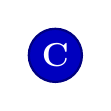
\begin{tikzpicture}[baseline=-0.6ex, scale=0.75]
    \draw[fill=blue!75!black, draw=blue!50!black, line width=0.8pt]
      (0,0) circle (0.45cm);
    \node[text=white, font=\bfseries\large] at (0,0) {C};
  \end{tikzpicture}%
}
\newcommand{\simboloClaseD}{%
  
\begin{tikzpicture}[baseline=-0.6ex, scale=0.75]
    \draw[fill=yellow!95!black, draw=yellow!60!black, line width=0.8pt]
      (90:0.60cm) -- (126:0.29cm) -- (162:0.60cm) -- (198:0.29cm) -- (234:0.60cm) --
      (270:0.29cm) -- (306:0.60cm) -- (342:0.29cm) -- (18:0.60cm) -- (54:0.29cm) -- cycle;
    \node[text=black, font=\bfseries\large] at (0,0) {D};
  \end{tikzpicture}%
}
\newcommand{\simboloClaseK}{%
  
\begin{tikzpicture}[baseline=-0.6ex, scale=0.75]
    \draw[fill=black!90!white, draw=black, line width=0.8pt]
      (30:0.48cm) -- (90:0.48cm) -- (150:0.48cm) -- (210:0.48cm) -- (270:0.48cm) -- (330:0.48cm) -- cycle;
    \node[text=white, font=\bfseries\large] at (0,0) {K};
  \end{tikzpicture}%
}

\begin{table}[!ht]
    \centering
    \begin{tabular}{|c|>{\centering\arraybackslash}m{2.8cm}|>{\raggedright\arraybackslash}m{5.4cm}|>{\raggedright\arraybackslash}m{4.8cm}|}
        \hline
        \textbf{Clase} & \textbf{Símbolo Normalizado} & \textbf{Materiales Involucrados} & \textbf{Agente Primario} \\ \hline
        A & \simboloClaseA & Madera, papel, telas, gomas, plásticos con brasa. &
        Agua presurizada, espuma AFFF, polvo ABC. \\ \hline
        B & \simboloClaseB & Líquidos inflamables, hidrocarburos, disolventes, gases. &
        Polvo químico ABC/BC, $CO_2$, espumas. \\ \hline
        C & \simboloClaseC & Instalaciones y circuitos eléctricos bajo tensión. &
        Dióxido de carbono ($CO_2$), polvo ABC/BC. \\ \hline
        D & \simboloClaseD & Magnesio, sodio, potasio, titanio, litio. &
        Polvos especiales secos (cloruro de sodio/grafito). \\ \hline
        K & \simboloClaseK & Aceites y grasas de cocina a altas temperaturas. &
        Solución química húmeda (acetato de potasio). \\ \hline
    \end{tabular}
    \caption{Clasificación normalizada de fuegos conforme a IRAM 3517 y NFPA 10.}
    \label{tab.cap2:clases_fuego}
\end{table}

\section{Efecto Joule y Teoría de Contactos}

En instalaciones eléctricas e industriales, la energía de activación inicial suele derivar de la disipación térmica
asociada a la corriente eléctrica. Conforme a la ley de Joule, la potencia térmica desarrollada en un conductor o
elemento resistivo responde a la ecuación \ref{eq.cap2:joule}:

\begin{equation}
\label{eq.cap2:joule}
P = I^2 \cdot R
\end{equation}

Donde $P$ representa la potencia disipada en watts, $I$ la corriente eficaz en amperes y $R$ la resistencia eléctrica en
ohms. En instalaciones adecuadamente proyectadas, las densidades de corriente se mantienen dentro de límites térmicos
seguros. No obstante, en bornes de conexión, barras colectoras y empalmes intervienen los fenómenos descritos por la
teoría de contactos eléctricos.

A escala microscópica, las superficies metálicas más pulidas presentan rugosidades pronunciadas. Por ende, la unión
física real ocurre exclusivamente en los puntos de contacto de las crestas o asperezas microscópicas,
de modo que el área de conducción efectiva suele representar menos del $1\percent$ del área aparente de la bornera.
Esta restricción geométrica de las líneas de flujo de corriente induce la denominada resistencia de constricción.

Con el transcurso del tiempo, los ciclos térmicos de carga y descarga provocan dilataciones y contracciones mecánicas
diferenciales. Este fenómeno genera una relajación paulatina en el par de apriete de los tornillos, reduciendo aún más el
área de contacto real y elevando la resistencia de constricción. Paralelamente, el incremento localizado de temperatura
acelera la oxidación superficial del cobre, conformando películas de óxido cuproso de naturaleza semiconductora y
aislante. Este proceso desencadena un círculo vicioso de desbocamiento térmico: al subir la temperatura, la resistividad
del metal y la capa de óxido aumentan, incrementando la resistencia global del contacto y la potencia térmica disipada,
hasta alcanzar la temperatura de ignición de las aislaciones poliméricas adyacentes.

\section{Fenómenos de Arco Eléctrico en Instalaciones}

Las fallas por arco eléctrico constituyen descargas disruptivas a través de un medio gaseoso ionizado, dando lugar a un
canal de plasma con temperaturas que sobrepasan los $6000\Celsius$. En instalaciones de baja tensión se presentan dos
configuraciones elementales:

\begin{itemize}
    \item Arco en Paralelo: Se establece entre dos conductores activos de distinta fase, o entre una fase y el neutro o
          conductor de puesta a tierra. Este evento origina corrientes de falla transitorias elevadas. Por lo general,
          estos niveles de corriente superan el umbral magnético de los interruptores termomagnéticos convencionales,
          permitiendo su desconexión en tiempos breves, excepto cuando la impedancia intrínseca del arco limita la
          corriente por debajo del umbral de disparo instantáneo.
    \item Arco en Serie: Ocurre a lo largo de la trayectoria de un mismo conductor activo debido a fisuras internas por
          fatiga, hebras cortadas o conexiones aflojadas. En este caso, la corriente de falla está estrictamente limitada
          por la propia impedancia de la carga conectada aguas abajo, manteniéndose en valores nominales de operación. Por
          este motivo, ni los interruptores termomagnéticos ni los protectores diferenciales detectan el siniestro,
          permitiendo que el plasma térmico permanezca activo de forma indefinida hasta incinerar los recubrimientos y
          estructuras circundantes.
\end{itemize}
